Skemaernes fitness er beregnet ud fra følgende værdier:
\begin{figure}[!h]
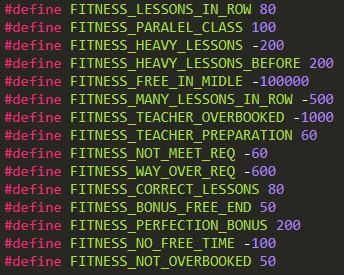
\includegraphics[width=\textwidth]{partials/graphics/fitness.png}
\caption{Billede over de fitness værdier skemaerne bliver tildelt, i tilfælde af at de opfylder visse parametre}
\label{fitnessvalues}
\end{figure}
De forskellige værdier kan godt give trække ned eller give positive versioner mere end en gang. Det vil sige at, hvis der er to steder på skemaet hvor der er en lærer der er overbooked giver det -2000 i fitness.
I den første test, undersøges det om fitnessen udregnes korrekt. De nedenstående skemaer er generet gennem softwareløsningen. De tre skemaer er alle skemaer for 7.B, de skal altså derfor alle have det samme antal af timer. 
I det første skema har 7.B alle det antal af timer de skal have, det kan ses på perfection grade 13, hvis de skemaet havde for lidt lektioner ville denne perfection grade blive lavere. Dette skema har dog for mange af nogle lektioner. Dette kan observeres i Must have og Have, hvor fagene står i følgende rækkefølge dansk, matematik, engelsk, tysk, fysik/kemi, historie, samfundsfag, valgfag, geografi, biologi, idræt, kristendom, praktiske fag og fri timer til sidst. I det første skema er der tre fag, hvor der er for mange lektioner, navnlig fysik, hvor der er en lektion for meget, geografi hvor der er to lektioner for meget og biologi hvor der er to for meget. Dette har negativ indflydelse på skemaet.
Skemaet positive fitness er en kombination af lessons with parallel, som er det antal af lektioner der foregår på samme tid som en af parallelklasserne. Dette skema har dog ingen lektioner på sammen tid med begge parallelklasser. Det der giver dette skema mindre i fitness, er at det har ’tunge’ fag som ligger over middag, nemlig 10. Derudover er lærerne også overbooked 3 gange i dette skema, det vil sige at der er tre tilfælde, hvor en af klassens lærer, har en eller flere lektioner på samme tid. Skemaets samlede fitness er 5961. 
\begin{figure}[!h]
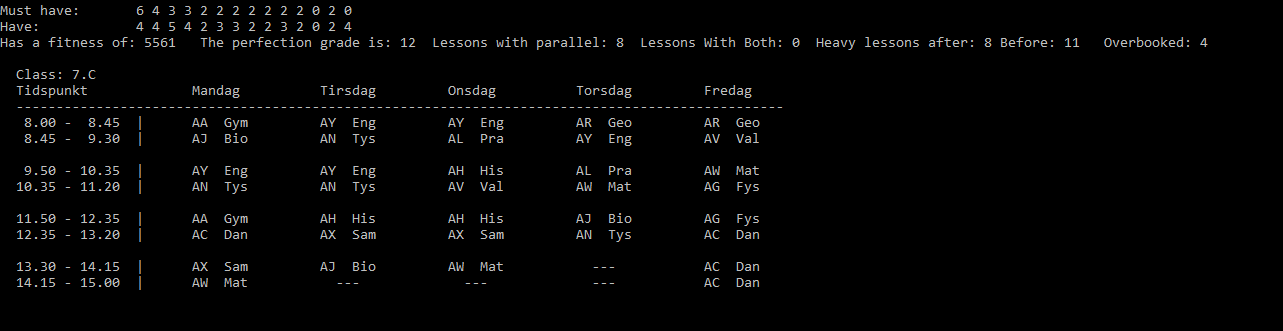
\includegraphics[width=\textwidth]{partials/graphics/fitness1.png}
\caption{Billede af et generet skema}
\label{fitness1}
\end{figure}

Det andet skema har også en perfction grade på 13, alle kravene for antallet fag er altså opfyldt. Der er dog to fag hvor der er en lektion for meget, faget for disse lektioner er engelsk, hvor der er en lektion for meget og geografi, hvor der er en lektion for meget. I skemaet er der ti fælles lektioner med parallel klasserne, der er dog kun 2 med begge parallelklasser. På skemaet er der ti lektioner med tunge fag over middag. Der er en lektion hvor en lærer har mere end en lektion på samme tidspunkt. Dette skemas samlede fitness er 8631.
\begin{figure}[!h]
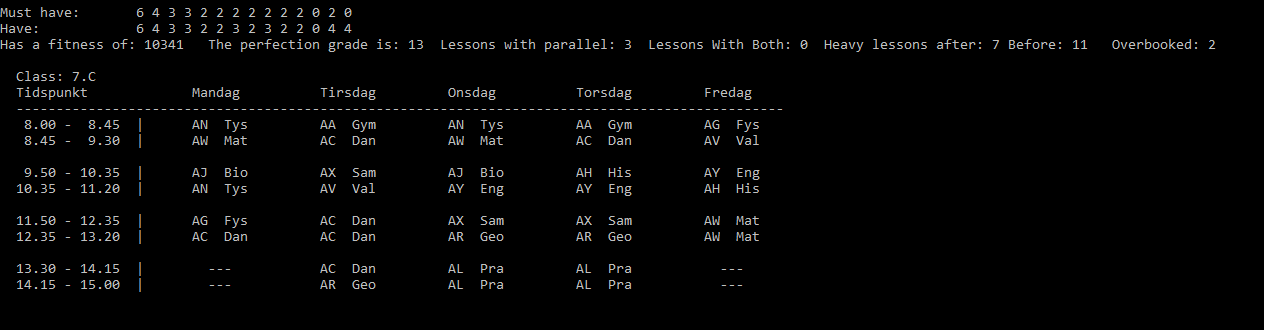
\includegraphics[width=\textwidth]{partials/graphics/fitness2.png}
\caption{Billede af et generet skema}
\label{fitness2}
\end{figure}

Perfection graden er også 13 i det tredje skema, der er altså ikke for lidt lektioner af nogle fag. Der er dog fire fag hvor der er for mange lektioner. Disse fag er dansk, hvor der er en lektion for meget, tysk, hvor der er en lektion for meget, geografi, hvor der er en for meget og biologi hvor der er en for meget. På dette skema er der fire lektioner, hvor der er mulighed for at samarbejde med en parallelklasse, der er dog ingen lektioner, hvor der er mulighed for at samarbejde med begge parallelklasser. På det tredje skema er der otte gange, hvor et tungt fag ligger over middag, dette er det mindste antal ud af de tre skemaer. Det forekommer ingen gang at lærerne i det tredje skema har to planlagte skemaer på samme tid. 
\begin{figure}[!h]
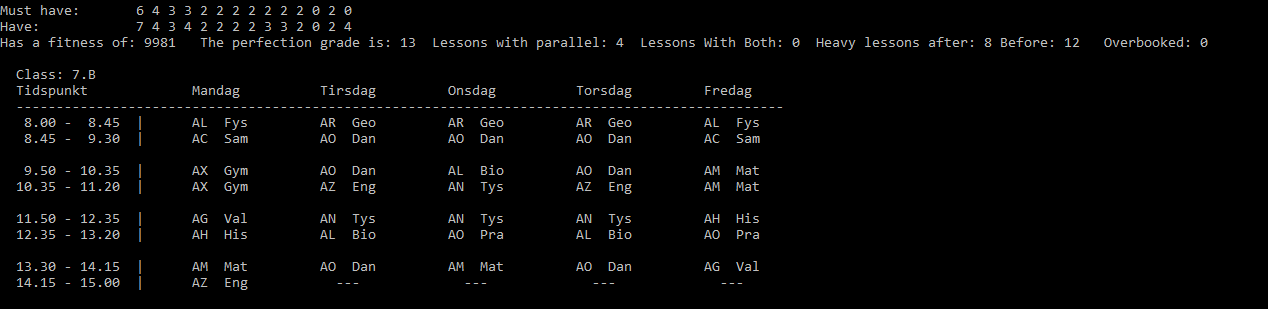
\includegraphics[width=\textwidth]{partials/graphics/fitness3.png}
\caption{Billede af et generet skema}
\label{fitness3}
\end{figure}

På tabellen med fitnessværdier, kan man se at fitnessværdien bliver trukket meget ned af have lærere der er ’overbooked,’ dette passer med at det tredje skema er det bedste da det ikke har nogle lærere der er ’overbooke.’ Derudover er det også den tredje der har mindst tunge lektioner over middag, hvilket også trækker de andre to skemaer ned. På det sidste skema er der dog ikke så meget mulighed for samarbejde på tværs af parallelklasserne. Dette kan dog skyldes at de andre to skemaer er har lærere der er ’overbooked,’ og derfor har lavet skemaet således at det er en ’overbooked’ lærer der har mulighed for at arbejde på tværs af parallelklasserne.
Ud fra tabellen med fitnessværdierne og undersøgelsen af de tre skemaer, kan det konkluderes at fitnessfunktionen fungerer som den skal. 
